\section{Auswertung}
\label{sec:Auswertung}
Die Fehlerrechnung dieses Kapitels genügt der gaußschen Fehlerfortpflanzung
\begin{equation}
  \label{eqn:Gauss}
  \Delta F = \sqrt{\sum_i\left(\frac{\symup{d}F}{\symup{d}y_i}\Delta y_i \right)^2}.
\end{equation}
%Die Standardfehler des Mittelwertes ergeben sich nach
%\begin{equation*}
%  \label{eqn:MW-Fehler}
%  \sigma(x) = \sqrt{\frac{1}{n(n-1)} \sum_i (x_i - \overline{x})^2}.
%\end{equation*}
Die Fehlerrechnung wird in \textit{Python} unter Verwendung des Paketes \textit{uncertainties} \cite{uncertainties} durchgeführt, jedoch werden die entsprechenden Fehlerformeln
an den jeweiligen Stellen angegeben.

\subsection{Bestimmung der Charakteristik des \textit{GMZ}}
\label{subsec:A_Charakteristik}
Um die Charakteristika des verwendeten Geiger-Müller-Zählrohres zu bestimmen werden die Messwerte aus \autoref{tab:Messwerte} verwendet.
Die Zählraten des \textit{GMZ} folgen einer Poissoin-Verteilung, weshalb sich die Unsicherheit der Messwerte $Z$ als $\symup{\Delta}Z = \sqrt{Z}$ annehmen lässt.
Nach Division durch die Messzeit $t = \qty{120}{\second}$ folgt die anschauliche und vergleichbare Größe $N$, die die Zählraten pro Zeiteinheit beschreibt.
Ihr Fehler ergibt sich nach \eqref{eqn:Gauss} zu 
\begin{equation*}
  \symup{\Delta}N = \frac{\sqrt{Z}}{\qty{120}{\second}}.
\end{equation*} 
Das Auftragen der zeitlich gemittelten Zählraten $N$ gegen die Spannung ergibt die charakteristische Kurve des \textit{GMZ}. Diese ist in \autoref{fig:plot}
dargestellt. Es lässt sich ein Bereich feststellen, in welchem die Kurve annähernd linear verläuft. Dieser ist mit grünen Messpunkten markiert. 

\begin{figure}
  \centering
  \includegraphics{plot.pdf}
  \caption{Messwerte der Charakteristik-Kurve des verwendeten Geiger-Müller-Zählrohres und lineare Ausgleichsgerade. Erstellt mit \textit{matplotlib} \cite{matplotlib}.}
  \label{fig:plot}
\end{figure}

Durch eine lineare Regression mittels \textit{scipy} \cite{scipy} folgen die Parameter
\begin{align*}
  a &= \qty{0.0125+-0.0022}{\volt^{-1}} & b &= \qty{104.4+-1.1}{\volt}
\end{align*}
der Ausgleichsgeraden $f(x) = ax + b$. Dies bedeutet eine Plateau-Steigung von $\qty{1.25+-0.22}{\percent}$. Die Länge des Plateaus ist die Differenz der äußersten Messpunkte,
welche zum Plateau gezählt werden. Sie lautet $L = \qty{270}{\volt}$

\subsection{Untersuchung der Nachentladung}
\label{subsec:Nachentladung}
Der zeitliche Abstand zwischen dem Primär- und Nachentladungsimpulsen kann über eine Betrachtung mit einem Oszilloskop bestimmt werden. Das dazu aufgenommene Bild wird in 
\autoref{fig:Oszilloskop} dargestellt. Aus der Abbildung kann entnommen werden, dass der Abstand zwischen dem Primär- und Nachentladungsimpulsen circa $\num{3.7}$ Kästchen 
in der \autoref{fig:Oszilloskop} beträgt. Ein Kästchen entspricht einem zeitlichen Abstand von $\qty{50}{\micro\second}$ daher liegen die Impulse um $\qty{185}{\micro\second}$
auseinander.
\begin{figure}
  \centering
  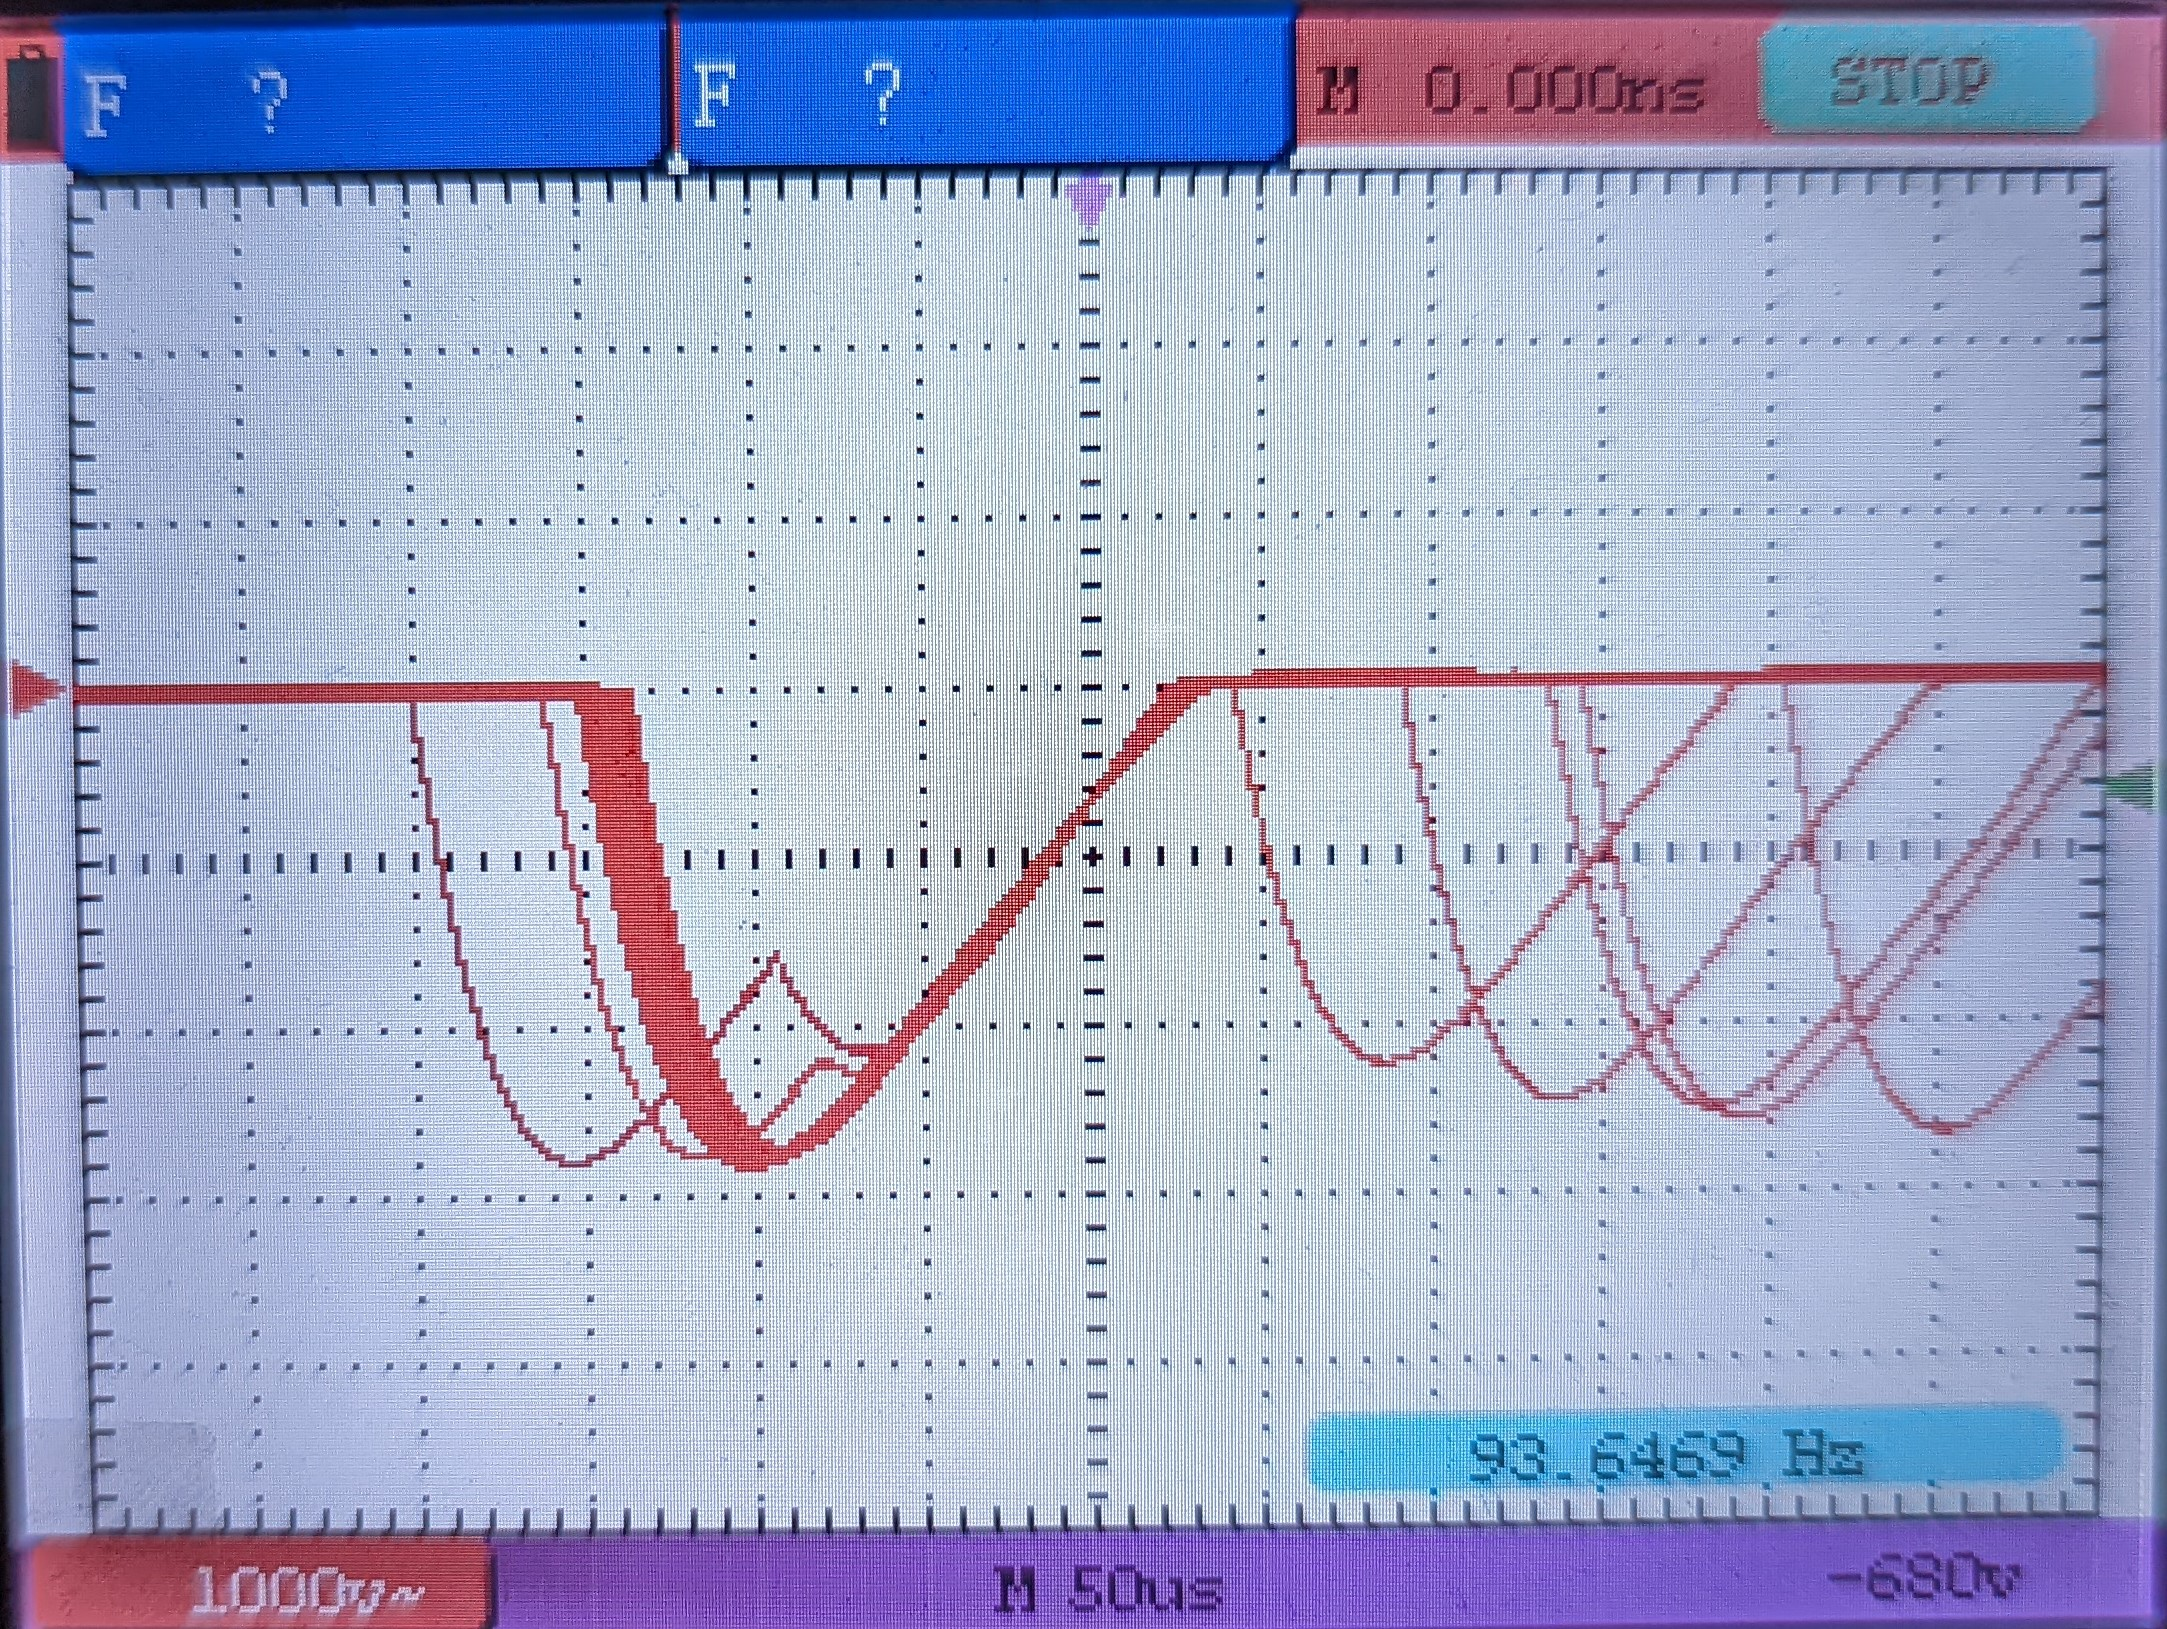
\includegraphics[width = .8\textwidth]{content/Oszilloskop_bild.jpg}
  \caption{In dieser Abbildung sind die Messdaten zur Nachentladung und zur Totzeit dargestellt, welche mittels eines Oszilloskops aufgenommen wurden.}
  \label{fig:Oszilloskop}
\end{figure}

\subsection{Bestimmung der Totzeit des Zählrohres}
\label{subsec:A_Totzeit}
Die Totzeit des verwendeten Zählrohres wird im folgendem über zwei Methode bestimmt. 
In der ersten Methode wird die Totzeit aus einer Messung mit einem Oszilloskops bestimmt. Die aufgenommen Messdaten sind in \autoref{fig:Oszilloskop} dargestellt.
Die Totzeit kann bestimmt werden durch den zeitlichen Abstand vom \textit{Hauptpeak} bis zu Punkt an dem dieser die Null erreicht. \autoref{fig:Oszilloskop} kann entnommen 
werden, dass dieser Abstand $\num{2.6}$ Kästchen entspricht. Daher folgt, äquivalent zum \autoref{subsec:Nachentladung}, dass die Totzeit über diese Methode 
$T = \qty{130}{\micro\second}$ beträgt.
Als zweite Methode wird die Zwei-Quellen-Methode verwendet. Bei einer Spannung $U = \qty{500}{\volt}$ und eine Messdauer von $\qty{120}{\second}$ wurde für den ersten 
$\beta$\,-Strahler eine Zählrate $N_1 = \num{20182 +- 142}$ gemessen. Der zweite $\beta$\,-Strahler Zählrate von $N_2 = \num{16262 +- 128}$. Die Messung beider 
Strahler zusammen ergab eine Zählrate von $N_{1+2} = \num{36370 +- 191}$. 
Die Totzeit kann gemäß 
\begin{equation}
  \label{eqn:Totzeit}
  T = \frac{N_1 + N_2 - N_{1+2}}{2N_1N_2}
\end{equation}
bestimmt werden. Mit der Zwei-Quellen-Methode ergibt sich eine Totzeit des Zählrohres von $T = \qty{13.53+-49.23}{\micro\second}$.

\begin{table}
  \centering
  \caption{Messwerte der charakteristischen Kurve des \textit{GMZ} und zur Bestimmung der freigesetzten Ladung. Es wurde jeweils für $t = \qty{120}{\second}$ gemessen.
          $U$ beschreibt die Spannung, $Z$ die Zählraten und $I$ den mittleren Strom. $N$ sind die Zählraten pro Sekunde mit Fehlerangabe.
          Die Unsicherheit der Strommesswerte beträgt $\qty{0.1}{\micro\ampere}$}
  \label{tab:Messwerte}
  \begin{tabular}{S[table-format = 3.0] S[table-format = 5.0] S[table-format = 3.1] @{${}\pm{}$} S[table-format = 1.2] S[table-format = 1.1]}
    \toprule{$U \mathbin{/} \unit{\volt}$} & {$Z$} & \multicolumn{2}{c}{$N \mathbin{/} \unit{\second^{-1}}$} & {$I \mathbin{/} \unit{\micro\ampere}$} \\
      \midrule
      320 & 12692 & 105.8 & 0.94 & 0.1 \\
      330 & 12881 & 107.3 & 0.95 & 0.2 \\
      340 & 12815 & 106.8 & 0.94 & 0.2 \\
      350 & 13066 & 108.9 & 0.95 & 0.2 \\
      360 & 13013 & 108.4 & 0.95 & 0.2 \\
      370 & 13008 & 108.4 & 0.95 & 0.2 \\
      380 & 13054 & 108.8 & 0.95 & 0.2 \\
      390 & 13055 & 108.8 & 0.95 & 0.2 \\
      400 & 13154 & 109.6 & 0.96 & 0.2 \\
      410 & 13094 & 109.1 & 0.95 & 0.2 \\
      420 & 13326 & 111.1 & 0.96 & 0.3 \\
      430 & 13082 & 109.0 & 0.95 & 0.3 \\
      440 & 13252 & 110.4 & 0.96 & 0.3 \\
      450 & 13144 & 109.5 & 0.96 & 0.3 \\
      460 & 13223 & 110.2 & 0.96 & 0.3 \\
      470 & 13247 & 110.4 & 0.96 & 0.4 \\
      480 & 13547 & 112.9 & 0.97 & 0.4 \\
      490 & 13222 & 110.2 & 0.96 & 0.4 \\
      500 & 13214 & 110.1 & 0.96 & 0.4 \\
      510 & 13297 & 110.8 & 0.96 & 0.4 \\
      520 & 13362 & 111.4 & 0.96 & 0.4 \\
      530 & 13292 & 110.8 & 0.96 & 0.4 \\
      540 & 13248 & 110.4 & 0.96 & 0.4 \\
      550 & 13481 & 112.3 & 0.97 & 0.5 \\
      560 & 13411 & 111.8 & 0.97 & 0.5 \\
      570 & 13111 & 109.3 & 0.95 & 0.5 \\
      580 & 13614 & 113.5 & 0.97 & 0.6 \\
      590 & 13223 & 110.2 & 0.96 & 0.6 \\
      600 & 13398 & 111.7 & 0.96 & 0.6 \\
      610 & 13468 & 112.2 & 0.97 & 0.6 \\
      620 & 13458 & 112.2 & 0.97 & 0.6 \\
      630 & 13768 & 114.7 & 0.98 & 0.6 \\
      640 & 13759 & 114.7 & 0.98 & 0.7 \\
      650 & 13494 & 112.5 & 0.97 & 0.7 \\
      660 & 13828 & 115.2 & 0.98 & 0.6 \\
      670 & 13811 & 115.1 & 0.98 & 0.7 \\
      680 & 14186 & 118.2 & 0.99 & 0.8 \\
      690 & 14039 & 117.0 & 0.99 & 0.8 \\
      700 & 14178 & 118.2 & 0.99 & 0.8 \\
    \bottomrule
  \end{tabular}
\end{table}

\subsection{Freigesetze Ladung des Zählrohres}
\label{subsec:Ladung}
Die freiwerdende Ladungsmenge $\mathrm{\Delta}Q$ kann aus der Formel \ref{eqn:Strom} durch umstellen nach $dQ$ errechnet werden. Daraus ergibt sich die Gleichung
\begin{equation}
  \mathrm{\Delta}Q = \frac{\overline{I}\mathrm{\Delta}t}{Ze}.
\end{equation}
Die daraus resultierenden Ladungswerte sind \autoref{fig:plot1} in Abhänigkeit von der Spannung zu entnehmen.

\begin{figure}
  \centering
  \includegraphics{plot1.pdf}
  \caption{In dieser Abbildung ist freigesetzte Ladungen des Zählrohres gegen die Spannung aufgetragen.}
  \label{fig:plot1}
\end{figure}